
%\keywords{Machine Learning Model Management; Stochastic Gradient Descent; Machine Learning Systems}

\section{Introduction} \label{introduction}
A machine learning pipeline consists of a set of data processing steps, chained together, that result in a machine learning model.
To fully utilize the model,  the model and the pipeline have to be deployed into an environment where they are used to answer prediction queries in real-time.
Typically, feedback in the form of new training data will become available based after the model is deployed.
In order to adapt to the new training data and guarantee a high prediction accuracy, new models are constantly trained and re-deployed.
Many platforms, e.g., Velox \cite{crankshaw2014missing}, Clipper \cite{crankshaw2016clipper}, Laser \cite{agarwal2014laser}, and TensorFlow Extended \cite{baylor2017tfx}, have been proposed to provide support for deployment and continuous training of machine learning pipelines. 
These platforms, either automatically or manually, facilitate the training and re-deployment of the models.
In many real-world use cases, training datasets are very large which makes training models that guarantee a high quality becomes a resource intensive and time consuming process.
Therefore, new models are trained periodically (typically daily).
This means that the model being used for answering prediction requests is not always up-to-date.
Online learning methods can be used to provide fresh and up-to-date models.
However, unless the online learning method used in training the model is highly tuned to the specific use case \cite{ma2009identifying}, a high quality model cannot be guaranteed.
This results in a trade-off between model quality and model freshness.

\begin{figure}[t]
\centering
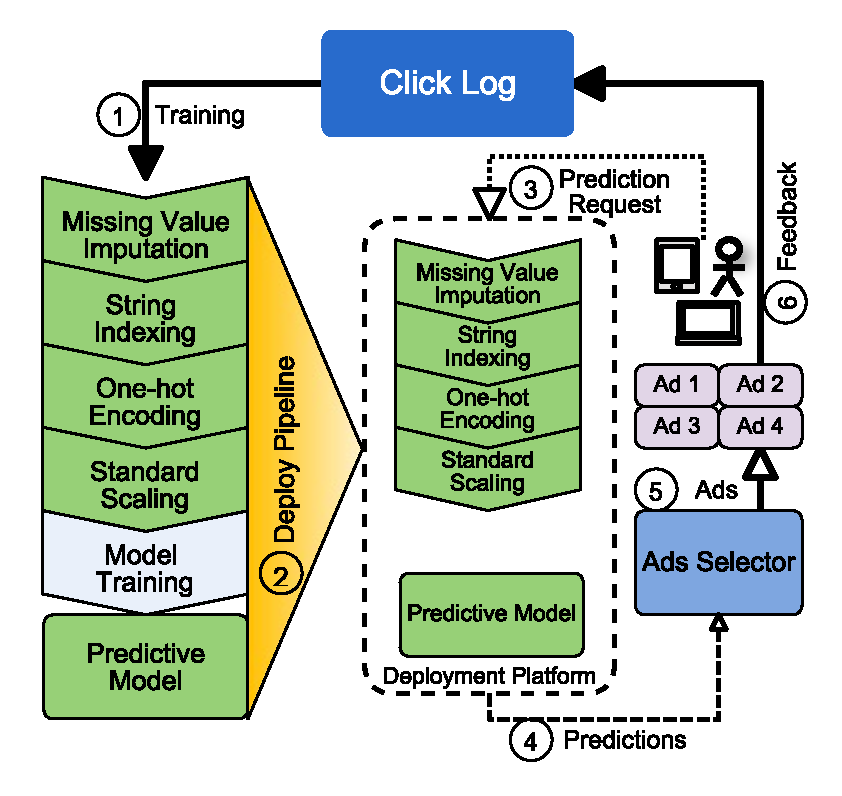
\includegraphics[width=\columnwidth]{../images/motivational-example.pdf}
\caption{Ads Serving Scenario}
\label{fig:motivational-example}
\end{figure}
\textbf{Example Application.} 
Online advertising is a multi-billion industry.
An advertising network receives ads from different businesses (ads providers) and shows them on different websites (publishers).
Typically, businesses are charged based on the number of clicks users make on their published ads.
Advertising networks use machine learning pipelines to estimate the click rate of different ads.
Figure \ref{fig:motivational-example} shows the work flow of an advertising firm.
The input data (Click Log) consists of several numerical and categorical variables related to the user, publisher's website,  the ads,  and whether or not the users clicked on those ads.
\textcircled{1} A basic click rate prediction pipeline contains the following components:
\begin{itemize}
\item A \textbf{missing value imputer} replaces missing values with appropriate values
\item A \textbf{label indexer} finds the different unique values in a categorical feature 
\item A \textbf{one-hot encoder} creates a new binary feature for every unique value in a categorical feature
%\item \hl{A \textbf{data bucketizer} transforms continuous variables into a series of binary variables}
\item A \textbf{standard scaler} scales the data columns to have unit standard deviation and zero mean
\item An finally a \textbf{logistic regression model} is trained using Stochastic Gradient Descent (SGD) optimization technique
\end{itemize}
The pipeline is trained on the click log dataset.
Once the pipeline is created, \textcircled{2} it is deployed into a platform to be used in production.
\textcircled{3} Whenever a user visits a publisher website, a series of prediction queries are sent to the deployment system where the pipeline is used to \textcircled{4} estimate the click rate of the user for the available ads on the website.
\textcircled{5} Ads with the highest click rate estimates are then shown to the user.
Depending on whether the user clicks on the ad or not, \textcircled{6} the platform generates new training data.
The new training data is combined with the existing click log.
Moreover, new users, new ads, and websites become available while the model is being served.
Therefore, the pipeline is periodically (typically on a daily basis) retrained using the data collected by the deployment platform.

The example above demonstrates the complex work flow of a deployment platform.
The deployment platform must be able to guarantee predictions with high accuracy and low latency.
This requires the platform to address the trade-off between quality and freshness.
Moreover, it must accommodates all the requests and new training data arriving at the system. 
Our goal is to design a deployment platform that can handle such traffic, provide more accurate predictions to the end user ,and provide a balance between model quality and model freshness.

\textbf{Existing Deployment methods.} 
To ensure high quality predictions, pipelines should be frequently updated.
However, existing solutions recognize training new models as a resource intensive and time consuming process \cite{crankshaw2014missing, agarwal2014laser, baylor2017tfx}.
To address the trade-off of quality and freshness, they propose periodical training of new models.
However, these periods are typically long (daily) and while they are appropriate for some use cases, they are not suitable for every use case.
This lead to high quality but out-of-date models.
Therefore, predictions made by the platform do not consider the most recent training data.
Moreover, in order not to stall the prediction query answering capabilities of the deployment platforms, batch training is performed outside of the deployment platform.
As a result, the information collected during the online processing is not available for the batch training. 

Existing solutions treat the training and deployment as two separate entities. 
As a result, models are first trained then pushed to the deployment environment.
We realized, by merging these two operations we can take advantage of the properties of the training method and update the model more rapidly without using extra resources.
This provides a balance between model freshness and model quality.
We call this approach proactive training.
Proactive training guarantees a higher average quality since the model is being updated constantly.
Moreover, by collecting statistics during the online processing of the data, we can speed up the training.
We propose a hybrid architecture for a deployment platform that updated the served models in-place and use the information collected while serving the model to speed up the training of the model.
The architecture enables for two key optimizations.
\todo[inline] {discuss SGD a bit more and fix the text so it makes sense}
\textit{Statistics collection. } 
We gather statistics during the online processing of the data. 
These statistics allow us to make the offline training more efficient since calculating them requires a complete scan of the entire dataset.
In our motivating example, label indexing, one-hot encoding, data bucketing, and standard scaling require statistics in form of the mean, standard deviation, and distribution of the features.

\textit{Proactive training.}
The underlying optimization technique (SGD) for the offline training is an iterative algorithm.
Individual iterations are independent and are typically light weight.
By exploiting these two features of SGD, we replace the time-consuming and resource intensive reactive batch training of the pipeline by a series of single iterations of SGD that are scheduled to execute proactively.
\hl{We provide a theoretical guarantee on how using SGD iterations can maintain the quality of the model.}

Our experiments show that proactive training of the pipelines achieves more accurate predictions overtime and requires less resources when compared to reactive retraining.

In summary our contributions are:
\begin{itemize}
\item A hybrid architecture for machine learning pipeline deployment platform that caters to both online and offline learning
\item Efficient training of the machine learning pipeline using statistics calculated during the online data processing
\item 
\item Removing the overhead of reactive offline training by replacing it with proactive mini-batch training
\end{itemize}

The rest of this paper is organized as follows:
Section \ref{continuous-training-serving} and \ref{sec:system-architecutre} introduce the design principles and architecture of our deployment system.
In Section \ref{evaluation}, we evaluate our system against different workloads and compare the performance of our method to other model deployment and maintenance approaches. 
Section \ref {related-work} discusses related work.
Finally, Section \ref{conclusion} presents our conclusion and future work.
%
%\begin{figure}[t]
%\centering
%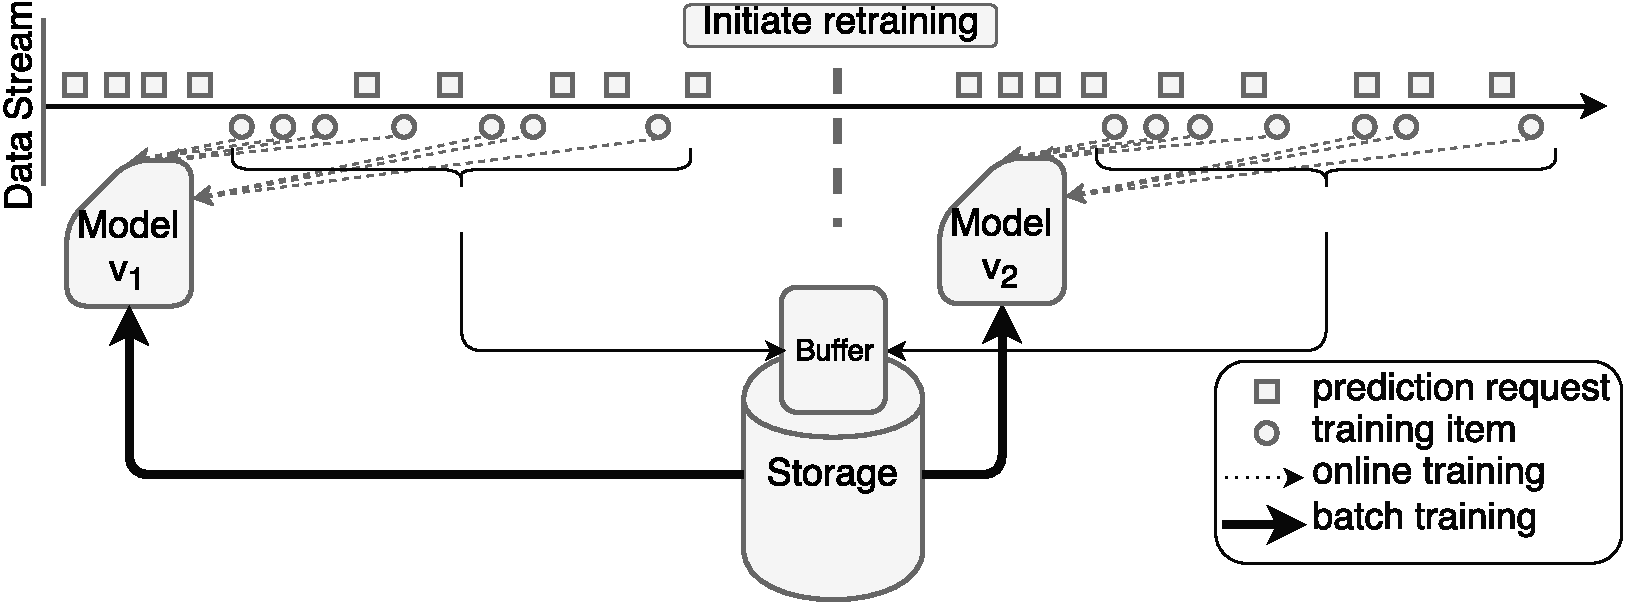
\includegraphics[width=1\columnwidth]{../images/velox-final.pdf}
%\caption{Current Model Deployment Method}
%\label{fig:velox-work-flow}
%\end{figure}


